\documentclass{standalone}
\usepackage{tikz}
\usetikzlibrary{patterns, positioning}


\begin{document}
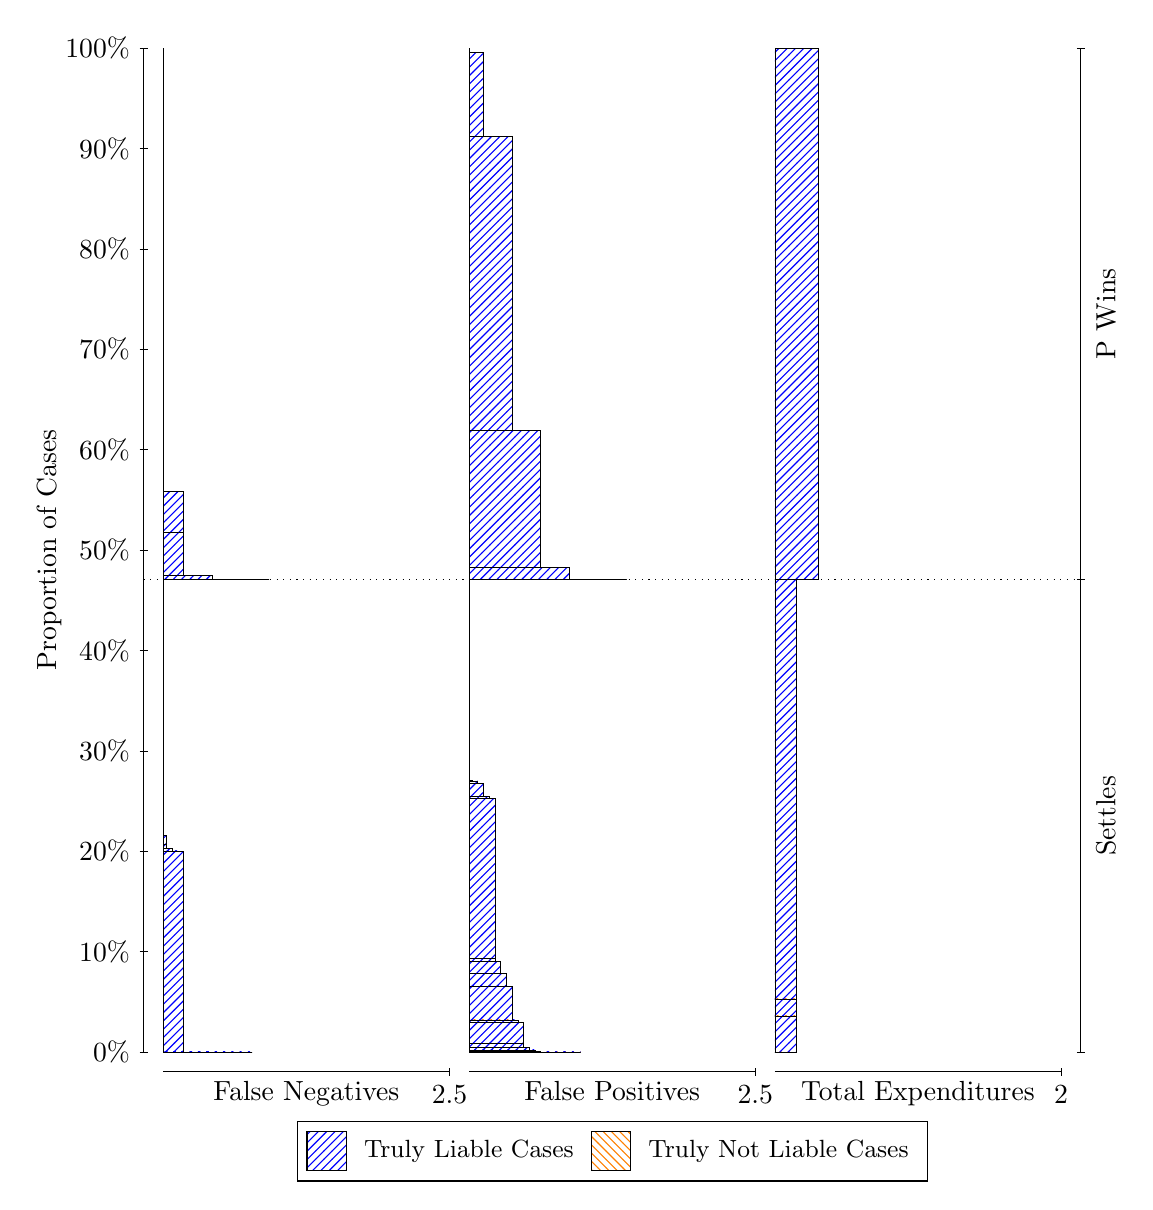
\begin{tikzpicture}
\draw[black, very thin] (1.5,1.75) -- (1.5,14.5);
\node[rotate=90, text=black, anchor=center] at (0.3, 8.125) {Proportion of Cases};
\draw[black, very thin] (1.45,1.75) -- (1.55,1.75);
\node[text=black, anchor=east] at (1.45, 1.75) {0\%};
\draw[black, very thin] (1.45,3.025) -- (1.55,3.025);
\node[text=black, anchor=east] at (1.45, 3.025) {10\%};
\draw[black, very thin] (1.45,4.3) -- (1.55,4.3);
\node[text=black, anchor=east] at (1.45, 4.3) {20\%};
\draw[black, very thin] (1.45,5.575) -- (1.55,5.575);
\node[text=black, anchor=east] at (1.45, 5.575) {30\%};
\draw[black, very thin] (1.45,6.85) -- (1.55,6.85);
\node[text=black, anchor=east] at (1.45, 6.85) {40\%};
\draw[black, very thin] (1.45,8.125) -- (1.55,8.125);
\node[text=black, anchor=east] at (1.45, 8.125) {50\%};
\draw[black, very thin] (1.45,9.4) -- (1.55,9.4);
\node[text=black, anchor=east] at (1.45, 9.4) {60\%};
\draw[black, very thin] (1.45,10.675) -- (1.55,10.675);
\node[text=black, anchor=east] at (1.45, 10.675) {70\%};
\draw[black, very thin] (1.45,11.95) -- (1.55,11.95);
\node[text=black, anchor=east] at (1.45, 11.95) {80\%};
\draw[black, very thin] (1.45,13.225) -- (1.55,13.225);
\node[text=black, anchor=east] at (1.45, 13.225) {90\%};
\draw[black, very thin] (1.45,14.5) -- (1.55,14.5);
\node[text=black, anchor=east] at (1.45, 14.5) {100\%};

\draw[black, very thin] (13.4,1.75) -- (13.4,14.5);
\draw[black, very thin] (13.35,1.75) -- (13.45,1.75);
\node[anchor=west] at (13.35, 1.75) {};
\draw[black, very thin] (13.35,7.7471) -- (13.45,7.7471);
\node[anchor=west] at (13.35, 7.7471) {};
\draw[black, very thin] (13.35,14.5) -- (13.45,14.5);
\node[anchor=west] at (13.35, 14.5) {};

\draw[black, very thin, pattern color=blue, pattern=north east lines] (1.75,1.75) rectangle (2.8763,1.75);
\draw[black, very thin, pattern color=blue, pattern=north east lines] (1.75,1.75) rectangle (2.731,1.75);
\draw[black, very thin, pattern color=blue, pattern=north east lines] (1.75,1.75) rectangle (2.5857,1.75);
\draw[black, very thin, pattern color=blue, pattern=north east lines] (1.75,1.75) rectangle (2.513,1.75);
\draw[black, very thin, pattern color=blue, pattern=north east lines] (1.75,1.75) rectangle (2.4403,1.75);
\draw[black, very thin, pattern color=blue, pattern=north east lines] (1.75,1.75) rectangle (2.3677,1.75);
\draw[black, very thin, pattern color=blue, pattern=north east lines] (1.75,1.75) rectangle (2.295,1.75);
\draw[black, very thin, pattern color=blue, pattern=north east lines] (1.75,1.75) rectangle (2.2223,1.7501);
\draw[black, very thin, pattern color=blue, pattern=north east lines] (1.75,1.7501) rectangle (2.1497,1.7504);
\draw[black, very thin, pattern color=blue, pattern=north east lines] (1.75,1.7504) rectangle (2.1497,1.7517);
\draw[black, very thin, pattern color=blue, pattern=north east lines] (1.75,1.7517) rectangle (2.077,1.7518);
\draw[black, very thin, pattern color=blue, pattern=north east lines] (1.75,1.7518) rectangle (2.0043,1.7521);
\draw[black, very thin, pattern color=blue, pattern=north east lines] (1.75,1.7521) rectangle (2.0043,4.2966);
\draw[black, very thin, pattern color=blue, pattern=north east lines] (1.75,4.2966) rectangle (1.9317,4.3035);
\draw[black, very thin, pattern color=blue, pattern=north east lines] (1.75,4.3035) rectangle (1.859,4.3375);
\draw[black, very thin, pattern color=blue, pattern=north east lines] (1.75,4.3375) rectangle (1.7863,4.3848);
\draw[black, very thin, pattern color=blue, pattern=north east lines] (1.75,4.3848) rectangle (1.7863,4.4969);
\draw[black, very thin, pattern color=orange, pattern=north west lines] (1.75,4.4969) rectangle (1.75,4.4969);
\draw[black, very thin, pattern color=blue, pattern=north east lines] (1.75,4.4969) rectangle (1.75,7.7471);
\draw[black, very thin, pattern color=blue, pattern=north east lines] (1.75,7.7471) rectangle (3.0943,7.7471);
\draw[black, very thin, pattern color=blue, pattern=north east lines] (1.75,7.7471) rectangle (2.731,7.7472);
\draw[black, very thin, pattern color=blue, pattern=north east lines] (1.75,7.7472) rectangle (2.3677,7.8001);
\draw[black, very thin, pattern color=blue, pattern=north east lines] (1.75,7.8001) rectangle (2.0043,8.3439);
\draw[black, very thin, pattern color=blue, pattern=north east lines] (1.75,8.3439) rectangle (2.0043,8.871);
\draw[black, very thin, pattern color=orange, pattern=north west lines] (1.75,8.871) rectangle (1.75,8.871);
\draw[black, very thin, pattern color=blue, pattern=north east lines] (1.75,8.871) rectangle (1.75,14.5);
\draw[black, very thin, pattern color=orange, pattern=north west lines] (5.6333,1.75) rectangle (7.0503,1.75);
\draw[black, very thin, pattern color=blue, pattern=north east lines] (5.6333,1.75) rectangle (7.0503,1.75);
\draw[black, very thin, pattern color=orange, pattern=north west lines] (5.6333,1.75) rectangle (6.905,1.75);
\draw[black, very thin, pattern color=blue, pattern=north east lines] (5.6333,1.75) rectangle (6.905,1.75);
\draw[black, very thin, pattern color=orange, pattern=north west lines] (5.6333,1.75) rectangle (6.7597,1.75);
\draw[black, very thin, pattern color=blue, pattern=north east lines] (5.6333,1.75) rectangle (6.7597,1.7502);
\draw[black, very thin, pattern color=blue, pattern=north east lines] (5.6333,1.7502) rectangle (6.687,1.7516);
\draw[black, very thin, pattern color=orange, pattern=north west lines] (5.6333,1.7516) rectangle (6.6143,1.7516);
\draw[black, very thin, pattern color=blue, pattern=north east lines] (5.6333,1.7516) rectangle (6.6143,1.7518);
\draw[black, very thin, pattern color=blue, pattern=north east lines] (5.6333,1.7518) rectangle (6.5417,1.7528);
\draw[black, very thin, pattern color=orange, pattern=north west lines] (5.6333,1.7528) rectangle (6.469,1.7528);
\draw[black, very thin, pattern color=blue, pattern=north east lines] (5.6333,1.7528) rectangle (6.469,1.7775);
\draw[black, very thin, pattern color=blue, pattern=north east lines] (5.6333,1.7775) rectangle (6.3963,1.8095);
\draw[black, very thin, pattern color=orange, pattern=north west lines] (5.6333,1.8095) rectangle (6.3237,1.8095);
\draw[black, very thin, pattern color=blue, pattern=north east lines] (5.6333,1.8095) rectangle (6.3237,1.8553);
\draw[black, very thin, pattern color=blue, pattern=north east lines] (5.6333,1.8553) rectangle (6.3237,2.1291);
\draw[black, very thin, pattern color=blue, pattern=north east lines] (5.6333,2.1291) rectangle (6.251,2.1575);
\draw[black, very thin, pattern color=orange, pattern=north west lines] (5.6333,2.1575) rectangle (6.1783,2.1575);
\draw[black, very thin, pattern color=blue, pattern=north east lines] (5.6333,2.1575) rectangle (6.1783,2.5902);
\draw[black, very thin, pattern color=blue, pattern=north east lines] (5.6333,2.5902) rectangle (6.1057,2.7476);
\draw[black, very thin, pattern color=blue, pattern=north east lines] (5.6333,2.7476) rectangle (6.033,2.902);
\draw[black, very thin, pattern color=blue, pattern=north east lines] (5.6333,2.902) rectangle (5.9603,2.9426);
\draw[black, very thin, pattern color=blue, pattern=north east lines] (5.6333,2.9426) rectangle (5.9603,4.9744);
\draw[black, very thin, pattern color=blue, pattern=north east lines] (5.6333,4.9744) rectangle (5.8877,5.0002);
\draw[black, very thin, pattern color=blue, pattern=north east lines] (5.6333,5.0002) rectangle (5.815,5.1595);
\draw[black, very thin, pattern color=blue, pattern=north east lines] (5.6333,5.1595) rectangle (5.7423,5.1935);
\draw[black, very thin, pattern color=blue, pattern=north east lines] (5.6333,5.1935) rectangle (5.6697,5.2004);
\draw[black, very thin, pattern color=blue, pattern=north east lines] (5.6333,5.2004) rectangle (5.6333,7.7471);
\draw[black, very thin, pattern color=orange, pattern=north west lines] (5.6333,7.7471) rectangle (7.6317,7.7471);
\draw[black, very thin, pattern color=blue, pattern=north east lines] (5.6333,7.7471) rectangle (7.6317,7.7471);
\draw[black, very thin, pattern color=orange, pattern=north west lines] (5.6333,7.7471) rectangle (7.2683,7.7471);
\draw[black, very thin, pattern color=blue, pattern=north east lines] (5.6333,7.7471) rectangle (7.2683,7.7493);
\draw[black, very thin, pattern color=orange, pattern=north west lines] (5.6333,7.7493) rectangle (6.905,7.7493);
\draw[black, very thin, pattern color=blue, pattern=north east lines] (5.6333,7.7493) rectangle (6.905,7.9085);
\draw[black, very thin, pattern color=orange, pattern=north west lines] (5.6333,7.9085) rectangle (6.5417,7.9085);
\draw[black, very thin, pattern color=blue, pattern=north east lines] (5.6333,7.9085) rectangle (6.5417,9.6408);
\draw[black, very thin, pattern color=orange, pattern=north west lines] (5.6333,9.6408) rectangle (6.1783,9.6408);
\draw[black, very thin, pattern color=blue, pattern=north east lines] (5.6333,9.6408) rectangle (6.1783,13.376);
\draw[black, very thin, pattern color=blue, pattern=north east lines] (5.6333,13.376) rectangle (5.815,14.447);
\draw[black, very thin, pattern color=blue, pattern=north east lines] (5.6333,14.447) rectangle (5.6333,14.5);
\draw[black, very thin, pattern color=orange, pattern=north west lines] (9.5167,1.75) rectangle (9.7892,1.75);
\draw[black, very thin, pattern color=blue, pattern=north east lines] (9.5167,1.75) rectangle (9.7892,2.2073);
\draw[black, very thin, pattern color=orange, pattern=north west lines] (9.5167,2.2073) rectangle (9.7892,2.2073);
\draw[black, very thin, pattern color=blue, pattern=north east lines] (9.5167,2.2073) rectangle (9.7892,2.4235);
\draw[black, very thin, pattern color=orange, pattern=north west lines] (9.5167,2.4235) rectangle (9.7892,2.4235);
\draw[black, very thin, pattern color=blue, pattern=north east lines] (9.5167,2.4235) rectangle (9.7892,7.7471);
\draw[black, very thin, pattern color=orange, pattern=north west lines] (9.5167,7.7471) rectangle (10.062,7.7471);
\draw[black, very thin, pattern color=blue, pattern=north east lines] (9.5167,7.7471) rectangle (10.062,14.5);
\draw[black, dotted] (1.5,7.7471) -- (13.4,7.7471);
\draw[black, very thin] (1.75,1.5) -- (5.3833,1.5);
\node[text=black, anchor=north] at (3.5667, 1.5) {False Negatives};
\draw[black, very thin] (5.3833,1.45) -- (5.3833,1.55);
\node[text=black, anchor=north] at (5.3833, 1.45) {2.5};

\draw[black, very thin] (5.6333,1.5) -- (9.2667,1.5);
\node[text=black, anchor=north] at (7.45, 1.5) {False Positives};
\draw[black, very thin] (9.2667,1.45) -- (9.2667,1.55);
\node[text=black, anchor=north] at (9.2667, 1.45) {2.5};

\draw[black, very thin] (9.5167,1.5) -- (13.15,1.5);
\node[text=black, anchor=north] at (11.333, 1.5) {Total Expenditures};
\draw[black, very thin] (13.15,1.45) -- (13.15,1.55);
\node[text=black, anchor=north] at (13.15, 1.45) {2};

\node[text=black, centered, rotate=90] at (13.72, 4.7485) {Settles};
\node[text=black, centered, rotate=90] at (13.72, 11.124) {P Wins};

\draw (7.449999999999999,1.5) node[draw=none] (baseCoordinate) {};
\begin{scope}[align=center]
        \matrix[scale=0.5, draw=black, below=0.5cm of baseCoordinate, nodes={draw}, column sep=0.1cm]{
            \node[rectangle, draw, minimum width=0.5cm, minimum height=0.5cm, pattern color=blue, pattern=north east lines] {}; &
            \node[draw=none, font=\small, text=black] (B) {Truly Liable Cases}; &
            \node[rectangle, draw, minimum width=0.5cm, minimum height=0.5cm, pattern color=orange, pattern=north west lines] {}; &
            \node[draw=none, font=\small, text=black] (B) {Truly Not Liable Cases}; \\
            };
\end{scope}

\end{tikzpicture}
\end{document}